\thispagestyle{empty}
\noindent
\strednp{
\NazovUniverzity\\
\NazovFakulty}
\vfill
\strednp{
\NazovDiela
%% \centerline{\PodazovDiela}
\mbox{}\\
\bigskip
\TypPrace
}
\vfill
\strednp{\textbf{\rok} \hfill{\textbf{\autor}}}
\newpage

\thispagestyle{empty}
\noindent
\strednp{\NazovUniverzity\\ \NazovFakulty}
\vfill
\strednp{\NazovDiela
%% \centerline{\PodazovDiela}
\mbox{}\\
\bigskip
\TypPrace
}
\vfill
\begin{tabular}{ l l }
\textbf{Študijný program:} & \program\\
\textbf{Študijný odbor:} & \cisloOdboru\ \odbor\\
\textbf{Školiace pracovisko:} & \katedra\\
\textbf{Vedúci práce:} &  \veduci
\end{tabular}
\bigskip\\
\bigskip\\
\bigskip\\
\bigskip\\
\strednp{\miestoRok \hfill{\autor}}
\newpage

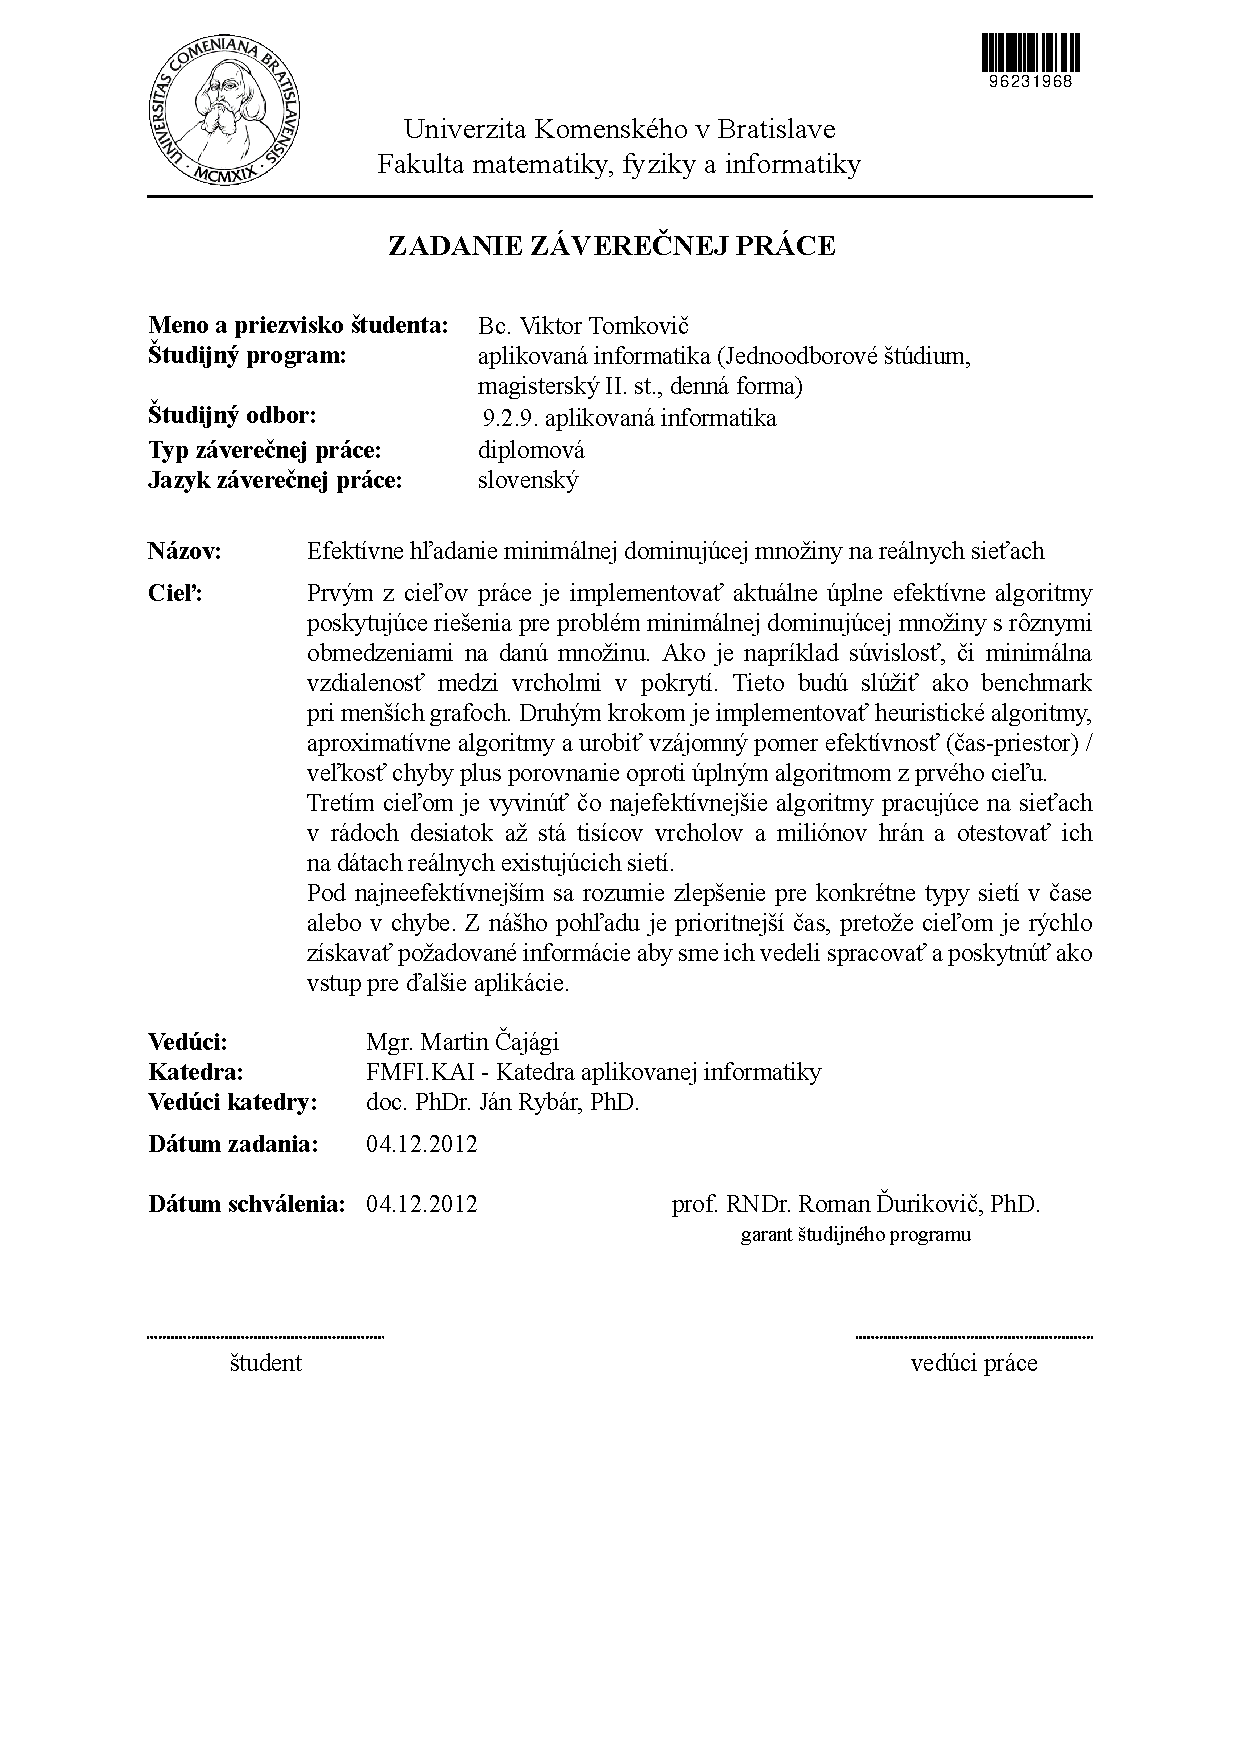
\includepdf[pages=1]{zadanie.pdf}

\newpage

\noindent
~\vfill

\section*{Poďakovanie}
Ďakujem.
\begin{comment}
Za odbornú pomoc, poskytnuté materiály a výborné vedenie pri tejto práci patrí 
veľká vďaka môjmu školiteľovi Martinovi Čajágimu. Taktiež by som sa chcel 
poďakovať mojim rodičom za pochopenie a poskytnuté možnosti vzdelávať sa.
\end{comment}
\\
\bigskip\\
\newpage

\chapter*{Abstrakt}
Táto práca skúma rôzne algoritmy na riešenie problému hľadania minimálnych
dominantných množín (MDS). Konkrétne skúma ich využitie v sieťach malého sveta.\\
Kľúčové slová: minimálna dominujúca množina, MDS, algoritmy a dátové štruktúry, siete 
malého sveta.

\newpage

\chapter*{Abstract}
This work is.\\
Keywords: minimal dominating set, MDS, algorithms and date structures, small-world 
network.
\newpage

\mbox{}
\newpage

\tableofcontents
\newpage
%\listoffigures
%\newpage
\listoftables
\newpage
